\documentclass[authoryear]{book}
\usepackage{graphics}
% or use the graphicx package for more complicated commands
\usepackage{graphicx}
\usepackage{pgf}
\usepackage{epsfig}
\usepackage{amssymb}
\usepackage{amsmath,latexsym}
\usepackage{array}
\usepackage[round]{natbib}
\usepackage{subfigure}
\usepackage{amsthm} %For theorems
 \usepackage{url}

\newcommand{\bm}[1]{\mbox{\boldmath $#1$}}


\theoremstyle{definition}
\newtheorem{theorem}{Theorem} %? [section]
\newtheorem{definition}[theorem]{Definition}
\newtheorem{question}{Question}
\newtheorem{answer}{Answer}


%\usepackage{Sweave}   
\usepackage{setspace} 
\setlength{\parindent}{0cm} 

\headsep=50pt
%\setlength{\parskip}{1.2ex}
\setlength{\parindent}{0.0mm}
\setlength{\textwidth}{16.5cm}
\setlength{\textheight}{23cm}
\setlength{\hoffset}{-0.8in}
\setlength{\voffset}{-1.3in}
\linespread{1.05}

\parindent=1.5pc
%\parskip=0pt
\setcounter{section}{0}
%\setcounter{tocdepth}{0}
% \setcounter{secnumdepth}{3}
%\textwidth=33pc
%\textheight=50pc
%\renewcommand{\figurename}{Fig.}

\def\Prob{\text{Prob}}
\def\E{\text{E}}
\def\Cov{\text{Cov}}
\def\Corr{\text{CoRrr}}
\def\Var{\text{Var}}
\def\Prec{\text{Prec}}
\def\R{\mathbb{R}}
\def\S{\mathbb{S}}


\def\mm#1{\ensuremath{\boldsymbol{#1}}} % version: amsmath
\def\MyFigureWidth{0.4\textwidth}
\def\MyFigureWidthTwo{9.5cm} %% 2*width + spacing
\def\MyFigureSpacing{6mm}

%%  To change the page layout from the default
%\addtolength{\topmargin}{-2cm}
%\addtolength{\textheight}{3cm}
%\addtolength{\oddsidemargin}{-0.5cm}
%\addtolength{\textwidth}{1cm}

% \SweaveOpts{width = 40}

\setkeys{Gin}{width=0.45\textwidth}

%\definecolor{links}{HTML}{2A1B81}
%\hypersetup{colorlinks,linkcolor=,urlcolor=links}

\def\SHS#1{\textcolor{blue}{SHS: #1}}
\def\JBI#1{\textcolor{green}{JBI: #1}}
\def\DB#1{\textcolor{red}{\textbf{DB: #1}}}

\title{Flexible spatial modelling with INLA and inlabru}

\author{Janine B Illian and others }

\date{\today}

\begin{document}
\maketitle

\chapter{Introduction to book}

\section{Introduction -- what is this book about}
Somebody who opens this book might wonder -- it this book for me? 
  
Many data sets with data structures that seem to be different initially.

Spatial component that has not been traditionally pointed out/discussed.

Motivate the diversity by showing examples

\section{Examples}



\subsection{Spatially continuous data}
% to do:
% find appropriate data set

\begin{figure}
\centering
%\includegraphics[width=0.3\textwidth]{complete}
%\includegraphics[width=0.6\textwidth]{sealsscotland}
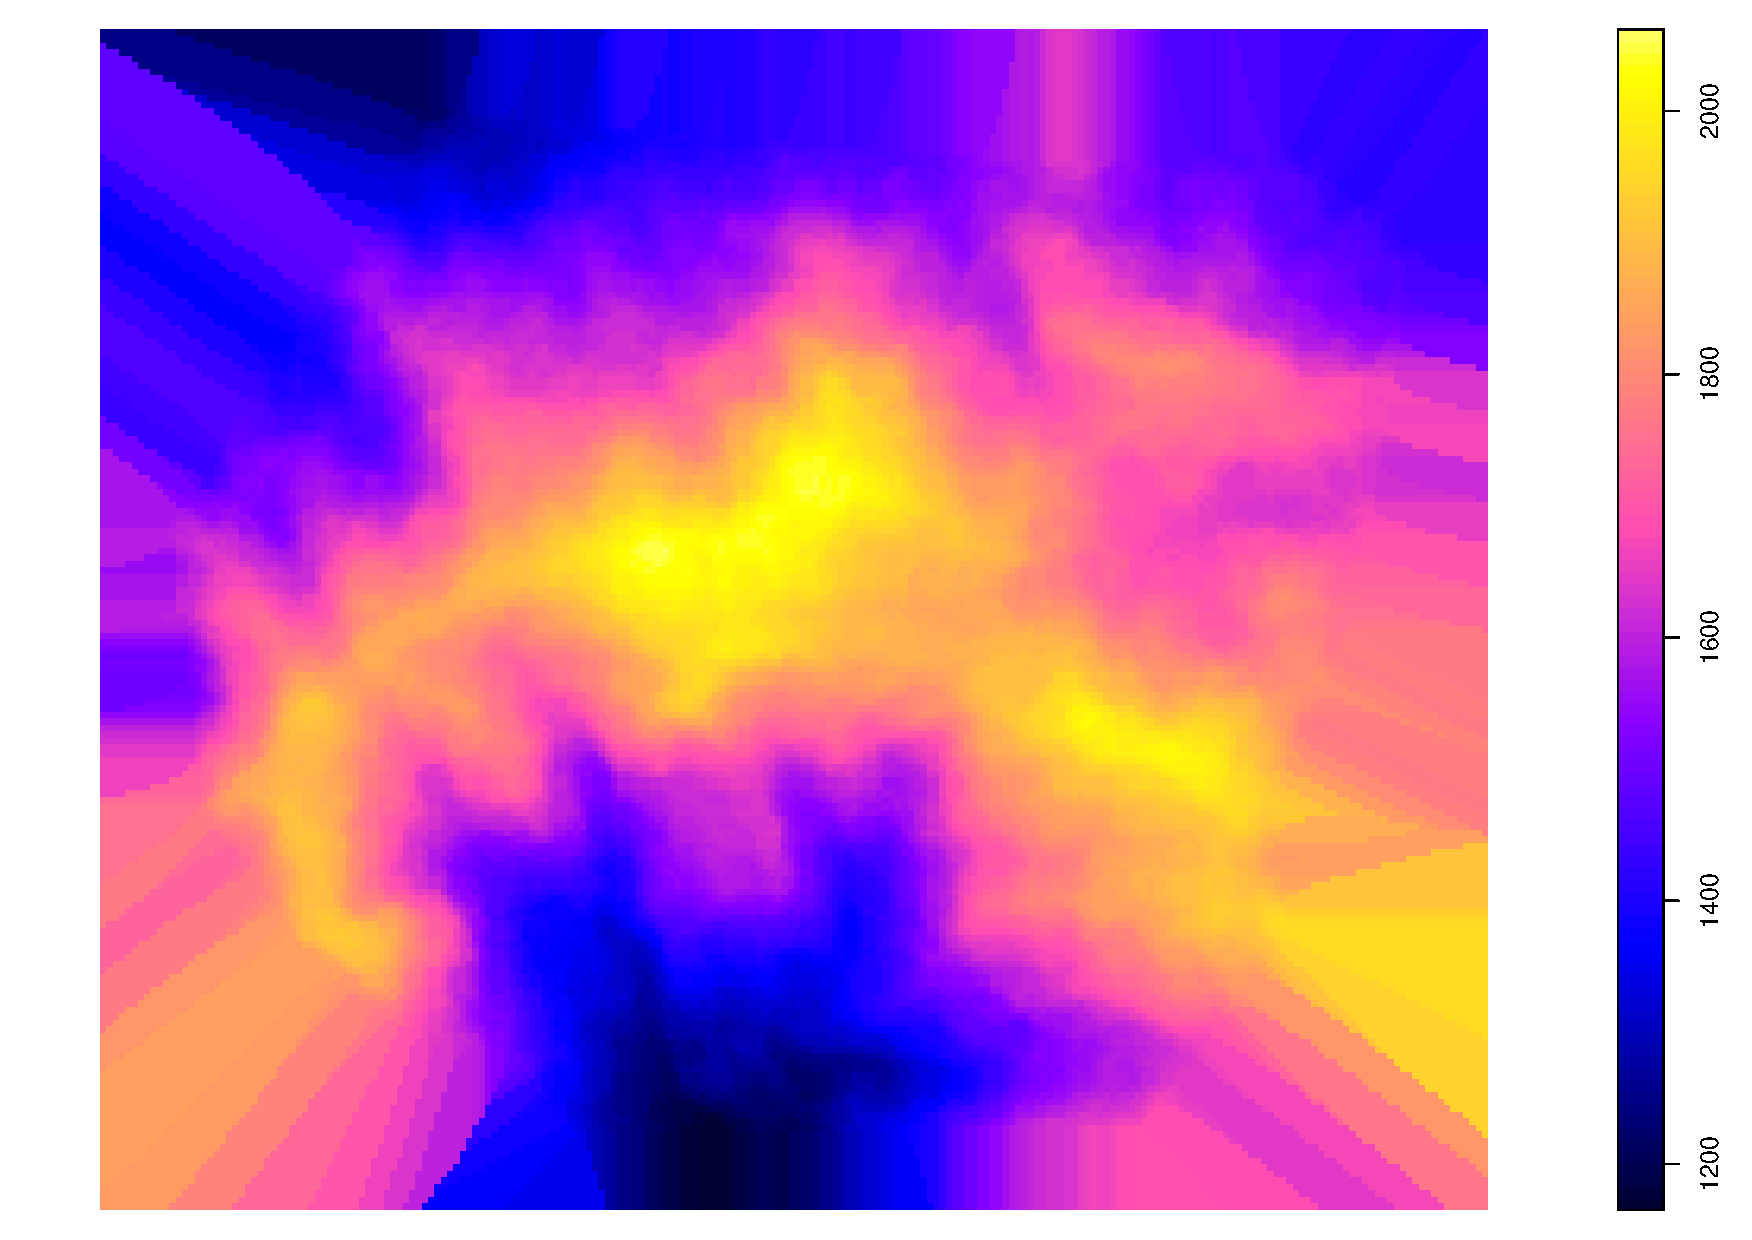
\includegraphics[width=0.6\textwidth]{elevation}
\caption{\label{fig:elev} Some elevation somewhere...}
\end{figure}




\subsection{Spatial point patterns}
\subsection{Data collected on transects}
\subsection{Distance sampling data}


\section{Synergy -- what do all these data sets have in common?  }

spatial structure

\section{What to expect from the book}

\end{document}



